\pagestyle{empty}
\chapter*{\centering \large DAFTAR RIWAYAT HIDUP}
\thispagestyle{empty}

\begin{wrapfigure}{l}{4cm}
	\vspace{-25pt}
	\begin{center}
		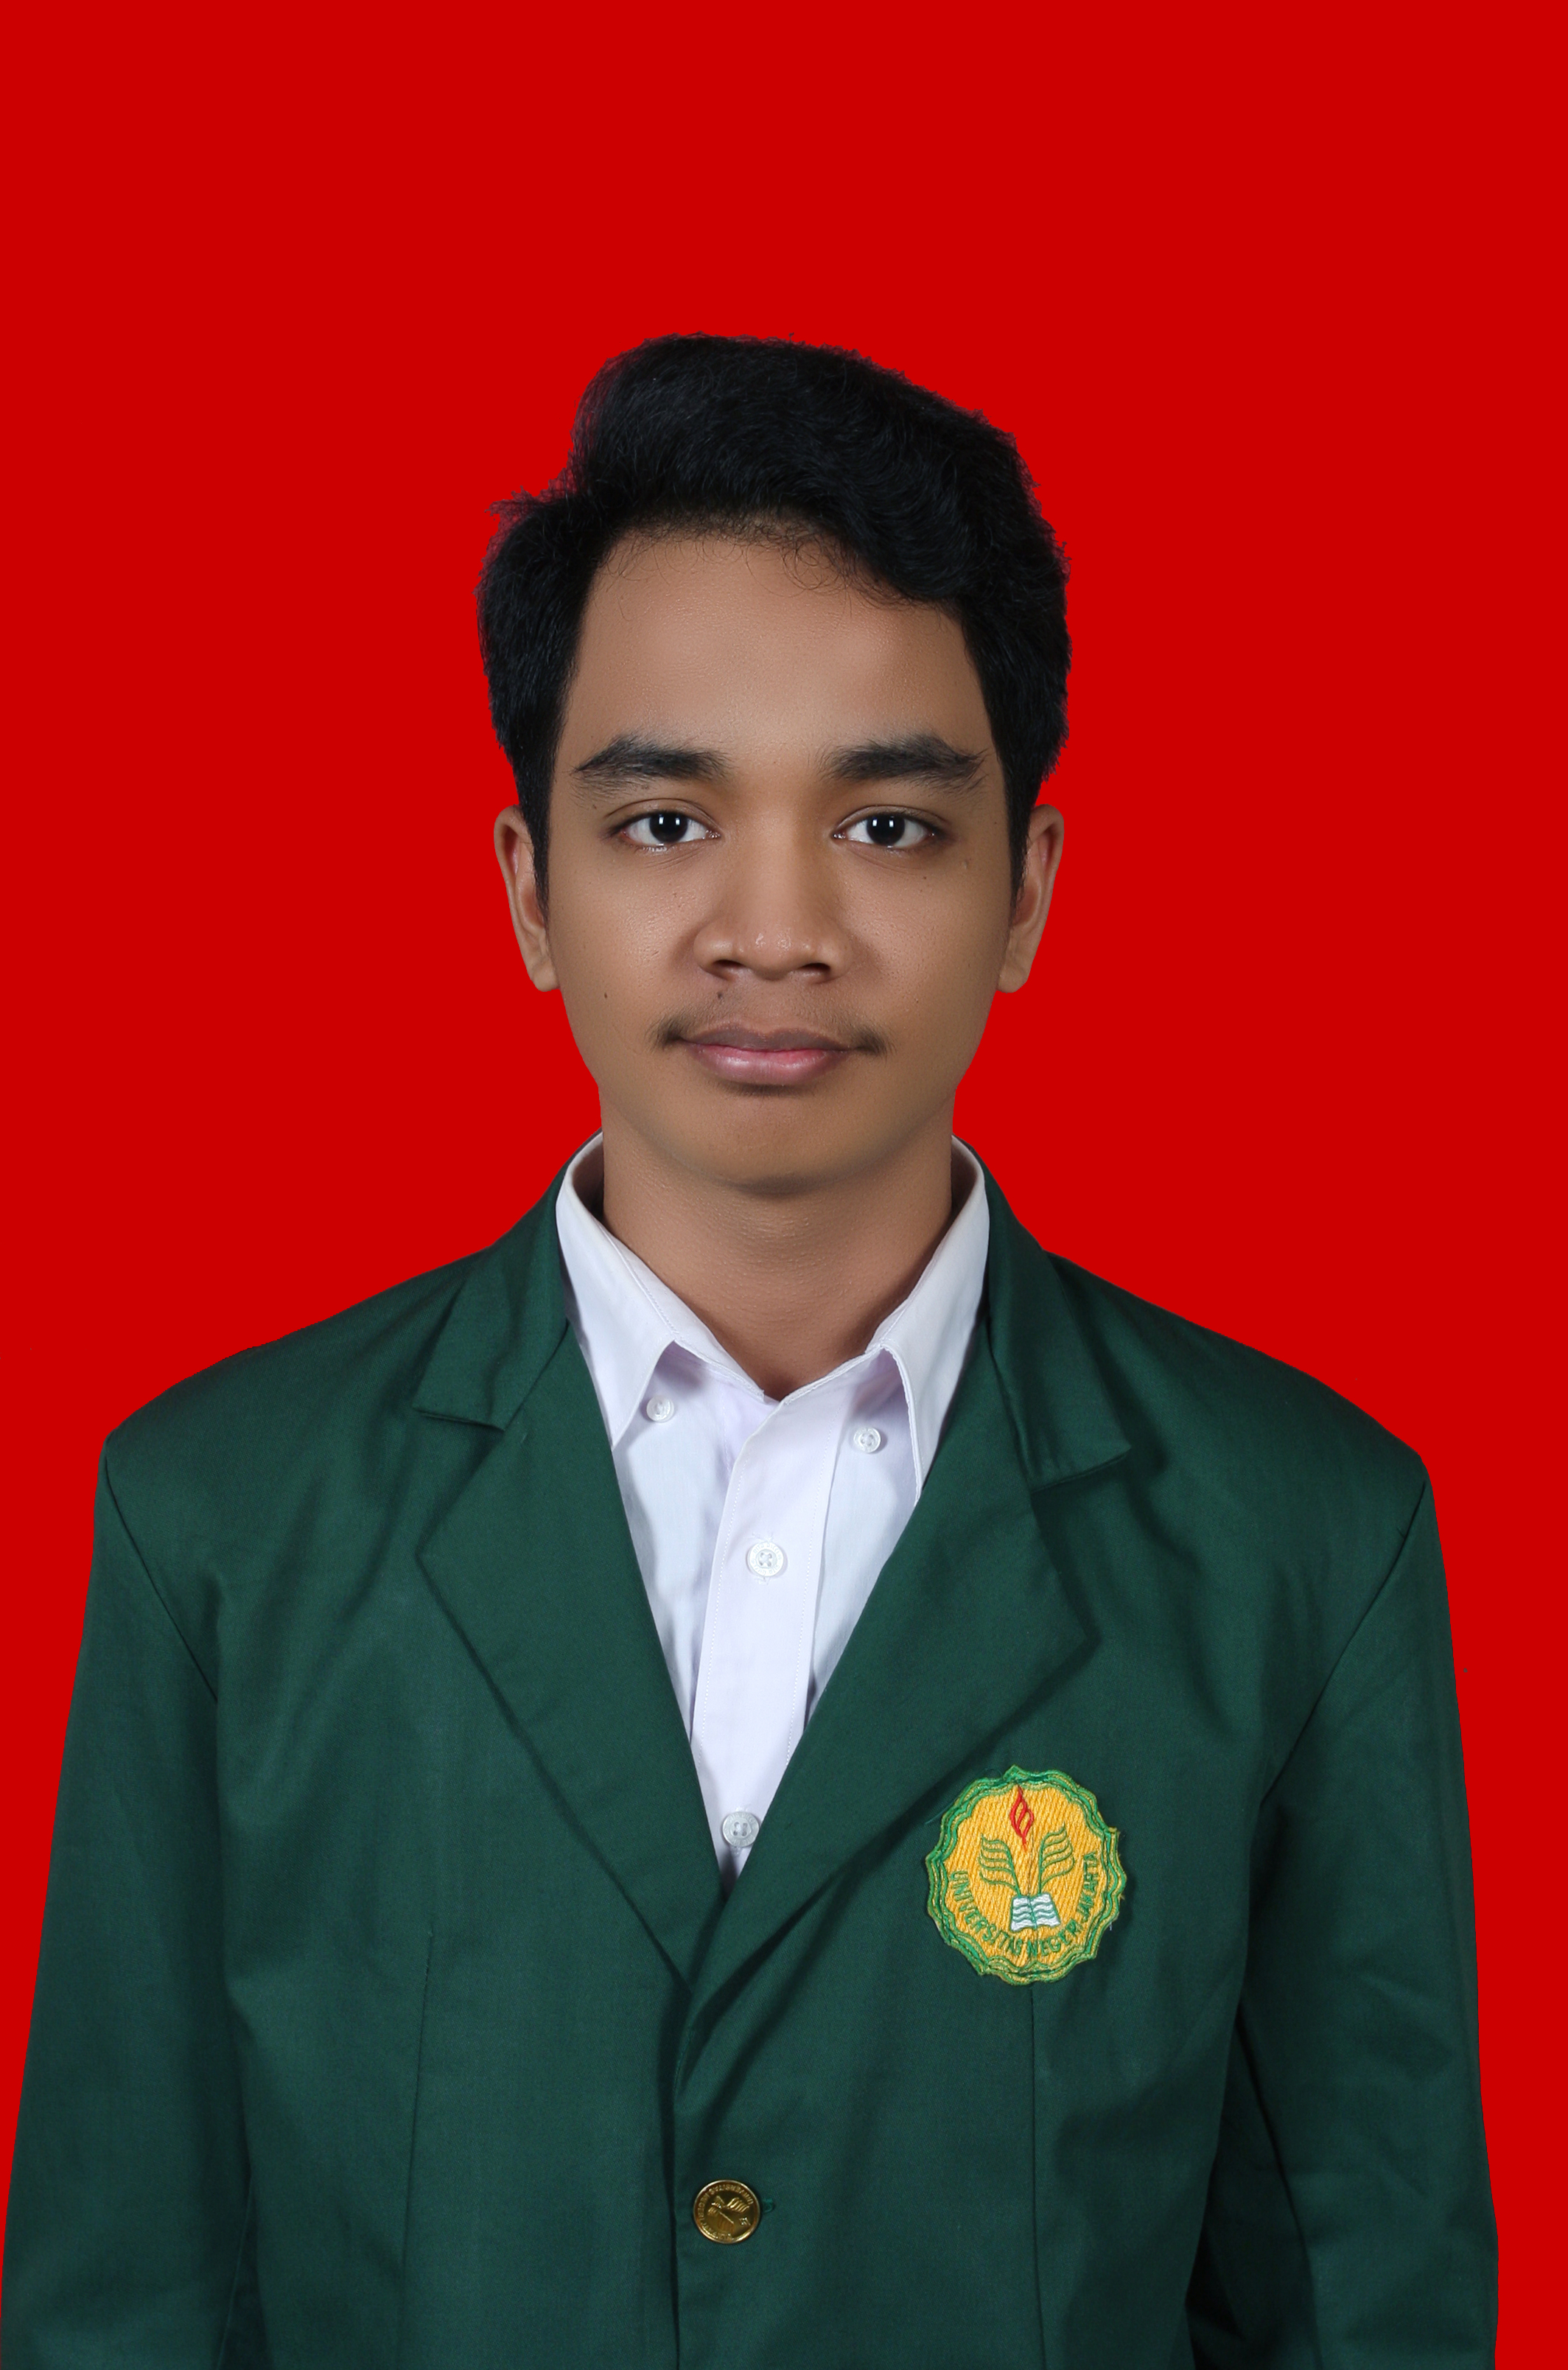
\includegraphics[width=0.27\textwidth]{gambar/12}
	\end{center}
	\vspace{-80pt}
\end{wrapfigure}

\noindent \textbf{ALDI RAHMANSYAH.}  Lahir di Jakarta, 9 Juni 1999.  Anak kedua dari pasangan Bapak Ahmad Dahlan (Alm) dan Ibu Lina Diah Wahyuni. Saat ini beralamatkan di Jl. Krakatau Blok 39/9 RT.007/RW.017 Perumahan Mekarsari, Cimanggis, Depok.

\vspace{0.5cm}
\noindent
\begin{center}
	\begin{flushright}
		\begin{tabular}{lcl}
			No. Ponsel	& :&  085156262082 \\
			Email	& :&  aldi.rahmansyah99@gmail.com
		\end{tabular}
	\end{flushright}
\end{center}
\vspace{0.5cm}

\noindent \textbf{Riwayat Pendidikan} : Penulis mengawali pendidikan di Raudhatul Ulum Jakarta Selatan pada tahun 2005-2006. Kemudian penulis berpindah ke SDN 03 Cibubur pada tahun 2006-2010. Setelah itu, penulis melanjutkan studi ke SMPN 91 Jakarta hingga tahun 2013. Kemudian melanjutkan ke SMAN 105 Jakarta pada tahun 2013-2016. Di Tahun 2016 penulis melanjutkan ke Universitas Negeri Jakarta (UNJ), Program Studi Ilmu Komputer, melalui jalur SNMPTN.

\noindent \textbf{Riwayat Organisasi} : Selama masa perkuliahan, penulis mengikuti organisasi DEFAULT periode 2018-2019 dan menjabat sebagai Wakil Ketua Bidang Divisi. Pada tahun 2018 juga, penulis melakukan penelitian dengan judul "Membandingkan Pengaruh Feature Selection Terhadap Algoritma Naïve Bayes Dan Support Vector Machine" yang dipublikasikan pada Seminar Nasional Aplikasi Teknologi Informasi (SNATi) dimana penulis menjadi pemakalah pembicara. Pada tahun yang sama penulis juga melakukan penelitian dengan judul "COPD detection 
using cough sound analysis based on machine learning" yang dipublikasikan pada Science and Mathematics International Conference (SMIC).